%Listing definition for Java
\definecolor{javared}{rgb}{0.6,0,0} % for strings
\definecolor{javagreen}{rgb}{0.25,0.5,0.35} % comments
\definecolor{javapurple}{rgb}{0.5,0,0.35} % keywords
\definecolor{javadocblue}{rgb}{0.25,0.35,0.75} % javadoc

\lstset{prebreak=\raisebox{0ex}[0ex][0ex]
        {\ensuremath{\rhookswarrow}}}
\lstset{postbreak=\raisebox{0ex}[0ex][0ex]
        {\ensuremath{\rcurvearrowse\space}}}
\lstset{breaklines=true, breakatwhitespace=true}
\lstset{numbers=left, numberstyle=\scriptsize}
 
\lstset{language=Java,
basicstyle=\ttfamily,
keywordstyle=\color{javapurple}\bfseries,
stringstyle=\color{javared},
commentstyle=\color{javagreen},
morecomment=[s][\color{javadocblue}]{/**}{*/},
numbers=left,
numberstyle=\tiny\color{black},
stepnumber=2,
numbersep=10pt,
tabsize=4,
showspaces=false,
showstringspaces=false
}

%%%%%%%%%%%%%%%%%%%%%%%%%%%%%%%%%%%%%%%%%%%%%%%%%%%%%%%%%%%%%%%%%%%%%%%%%%%%%

\chapter{Requirements}

This chapter covers the software requirements for the two modules this thesis is composed of. They are based on the recommendations provided by the scientists working on the ESTCube-1 project. The chapter is organised in three sections, the first one being the requirements which are common to both modules whereas the following two  go through each module's requirements more in depth.


\section{Common information for both modules}

\subsection{General Description}
\subsubsection{Product Perspective}
The modules are part the Hummingbird project based on the advise and needs dictated by the ESTCube-1 team members. For more information about Hummingbird see Chapter 3 and for more information about ESTCube-1 see Chapter 1. 

\subsubsection{General Constraints}

\begin{itemize}
\item The modules must be licenced under \textbf{Apache License v2.0} \cite{AL20}.
\item The use of open source tools is recommended.
\item The main programming language must be Java \cite{Java}.
\end{itemize}

\subsection{External Interface Requirements}

\subsubsection{Software Interfaces}

\textbf{\emph{Parameter}}\\
The modules will receive Parameters. The \emph{Parameter} type is part of Hummingbird and is represented as follows.

\begin{itemize}
\item Numeric value (can be any type).
\item Unit of the value.
\item Description: additional information about the parameter.
\item Timestamp: date and time when the parameter was created.

\end{itemize}


\textbf{\emph{Apache Camel}} \citep{Camel}\\
Since Hummingbird uses \emph{Apache Camel} for the communication between modules, the parameters for calibration are received and sent back using this system. In addition, Hummingbird has a heartbeat service to check if the module is responding properly. It is necessary to configure the module so it sends and receives messages through Camel.


\subsubsection{Communications Interfaces}

\textbf{\emph{JMS}} \cite{JMS}\\
The communication interface with the other components in the system is the Java Message Service using Apache Camel. The module is a \textbf{JMS client} in a \textbf{publish/subscribe model}.

\subsection{Non-Functional Requirements}

%\textbf{Performance}\\
\textbf{Reliability}\\
The software should handle unexpected values correctly. Eg. the value of the parameter is \emph{null} or \emph{NaN}.

\textbf{Availability}\\
Hummingbird setup can work without the modules. However, they must run for days without problems.

\textbf{Security}\\
Handled by Hummingbird.

\textbf{Maintainability}\\
XML configuration at startup.

\textbf{Portability}\\
Since it is written in Java it should work wherever a JVM is available.

\section{Calibration module}

\subsection{Introduction}

\subsubsection{Scope}

This software is intended to serve as an independent calibration module for \emph{Hummingbird}. As such, it will receive parameters with raw values, calibrate those values and generate new parameters which will be available for other modules in the system to use. The system must be flexible and allow users to define their own calibration scripts.

\subsubsection{Definitions}

\begin{itemize}
\item \textbf{Engineering values}: result of the calibration process.
\item \textbf{Raw values}: values received from the satellite, before going through the calibration process.
\item \textbf{Hummingbird:} see Chapter 3.
\end{itemize}

\subsection{General Description}
\subsubsection{Product Perspective}

Common to both modules. Please see the section 4.1.1.

\subsubsection{Product Functions}

\begin{itemize}
\item Information input
\begin{itemize}
\item Allow the user to input the calibration information as an XML file.
\item Parse the XML configuration to generate the calibration scripts.
\end{itemize}
\item Calibration process
\begin{itemize}
\item Receive one raw parameter and return one calibrated parameter.
\item Receive one raw parameter and return several calibrated parameters.
\item Receive several raw parameters and return one calibrated parameter.
\item Receive several raw parameters and return several calibrated parameters.
\end{itemize}

\end{itemize}

\subsubsection{User Characteristics}

\begin{itemize}
\item Specialists/Scientists
\begin{itemize}
\item Frequency of use: at the moment of inserting the calibration information.
\item Functions used: XML file to insert the calibration information. Other than that, the process is automated.
\item Technical expertise: Comfortable with XML and shell scripting. Also with simple Java programming.
\end{itemize}
\end{itemize}


\subsubsection{General Constraints}

Common to both modules. Please, see section 4.1.1.

\subsubsection{User Documentation}
\begin{itemize}
\item Manual for specialist/scientists who will be writing the calibration scripts. The manual must contain examples of the XML format and the way of representing the calibration scripts.
\end{itemize}

\subsection{External Interface Requirements}

\subsubsection{Software Interfaces}

In addition to receiving Parameters this module also generates and sends them. For more information see the section 4.1.2 as the interface is common for both modules.


\subsubsection{Communications Interfaces}

Common to both modules. Please see section 4.1.2

\pagebreak

\subsection{Functional Requirements}

\subsubsection{Read configuration}

\textbf{\emph{Introduction}}\\
The first thing the software should do is parse the configuration files to generate the calibration information.\\

\textbf{\emph{Inputs}} \linebreak
XML files with calibration information for the different subsystems.\\

\textbf{\emph{Processing}}\linebreak
\begin{enumerate}
\item Find XML files in the selected location.
\item Find calibration information available in each file.
\item Generate calibration table.
\end{enumerate}
\vspace*{1\baselineskip}


\textbf{\emph{Outputs}}\linebreak
The process will generate a table with the calibration information for all the different parameters.\\

%\textbf{\emph{Error Handling}}\\



\subsubsection{Listen to incoming parameters}

\textbf{\emph{Introduction}}\linebreak
The module will be waiting for new parameters to arrive. When a parameter is ready for calibration it will be sent to the calibrator.\\

\textbf{\emph{Inputs}}\linebreak
Parameters received through \emph{Apache Camel}.\\

\textbf{\emph{Processing}}\linebreak
\begin{enumerate}
\item Receive a parameter.
\item If the parameter is ready for calibration send it to the calibrator.
\item If the parameter needs more parameters to be calibrated wait for those parameters.
\end{enumerate}
\pagebreak
\textbf{\emph{Outputs}}\linebreak
The output will be one or several parameters which will be sent back to the message queue using \emph{Apache Camel}.\\


\textbf{\emph{Error Handling}}\\
\begin{itemize}
\item If no calibrator is found for the parameter log the error and ignore it. No data return to \emph{Apache Camel} is expected.
\item If there is a problem with the calibrator log the error and do not return any data through \emph{Apache Camel}.
\end{itemize}

\vspace*{1\baselineskip}
\subsubsection{Calibrate}

\textbf{\emph{Introduction}}\linebreak
When a parameter is ready for calibration it must be sent to the calibrator, including any extra parameters needed for the calibration and also the calibration information.\\

\textbf{\emph{Inputs}}\linebreak
Parameter to be calibrated plus all extra parameters needed to do so.\\

\textbf{\emph{Processing}}\linebreak
\begin{enumerate}
\item Receive parameter(s) needed for calibration.
\item Receive all the calibration information.
\item Use the script to generate the new value.
\item Return the new parameter.
\end{enumerate}
\vspace*{1\baselineskip}
\textbf{\emph{Outputs}}\linebreak
The output will be one or several parameters.\\


\textbf{\emph{Error Handling}}\\
If there is an error it must be sent upwards.\\

\pagebreak
\subsection{Non-Functional Requirements}

Common to both modules. Please see section 4.1.3.

\section{Limit checking module}

\subsection{Introduction}

\subsubsection{Scope}

This software is intended to serve as an independent limit checking module for \emph{Hummingbird}. It will receive a parameter and return information about the state of that parameter in relation to the limits.

\subsubsection{Definitions}

\begin{itemize}
\item \textbf{Hummingbird:} see Chapter 3.
\item \textbf{Parameter}: contains the value.
\item \textbf{State}: a boolean value reporting the state of the parameter.
\end{itemize}

\subsection{General Description}
\subsubsection{Product Perspective}

Common to both modules, please see the section 4.1.1.

\subsubsection{Product Functions}

\begin{itemize}
\item Information input
\begin{itemize}
\item Allow the user to input the limit checking information as an XML file.
\item Parse the XML configuration to generate the limits.
\end{itemize}


\end{itemize}

\subsubsection{User Characteristics}

\begin{itemize}
\item Specialists/Scientists
\begin{itemize}
\item Frequency of use: at the moment of inserting the limit checking information.
\item Functions used: XML file to insert the limit checking information. Other than that, the process is automated.
\item Technical expertise: Comfortable with XML.
\end{itemize}
\end{itemize}


\subsubsection{General Constraints}

In addition to the constraints common to both modules (see section 4.1.1) there must be two options:

\begin{itemize}
\item Sanity limits, soft limits and hard limits. (See Figure \ref{f4.2}).
\begin{figure}[H]
\centerline{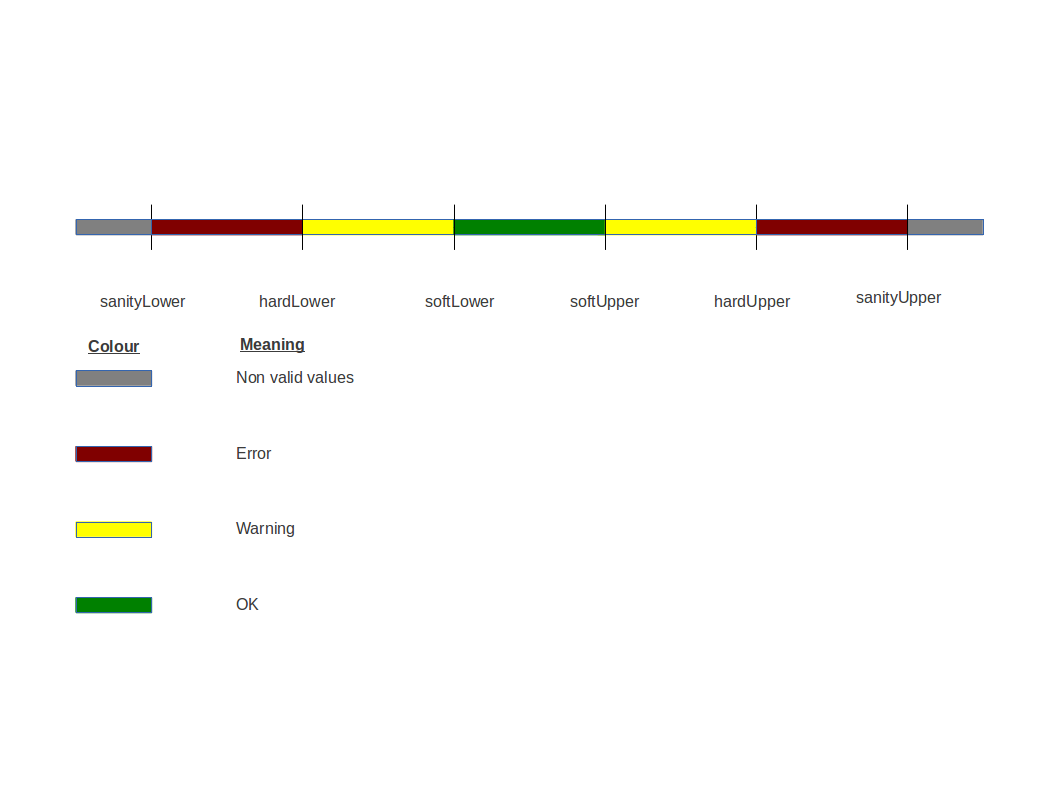
\includegraphics[width=1.2\textwidth]{images/LimitChecking1.png}}
\caption{Limit checker with sanity limits available}
\label{f4.2}
\end{figure}
\pagebreak
\item Soft limits and hard limits only (Figure \ref{f4.3}).
\begin{figure}[H]
\centerline{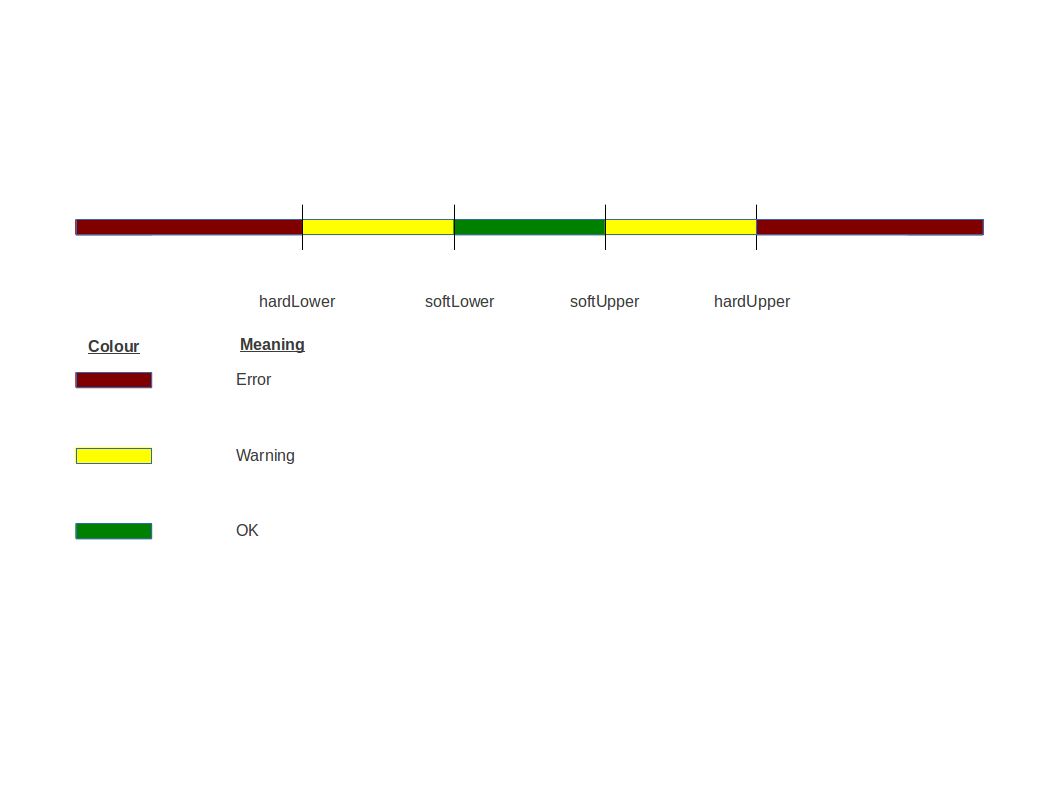
\includegraphics[width=1.2\textwidth]{images/LimitChecking2.png}}
\caption{Limit checker only with soft and hard limits}
\label{f4.3}
\end{figure}
\end{itemize}

\subsubsection{User Documentation}
\begin{itemize}
\item Manual for specialist/scientists who setting up the limits. The manual must contain examples of the XML format.
\end{itemize}
\pagebreak
\subsection{External Interface Requirements}

\subsubsection{Software Interfaces}

In addition to the common software interfaces for both modules (see section 4.1.2) there is one more software interface to be taken into account.

\textbf{\emph{State}}

The module will return States. The \emph{State} type is part of Hummingbird and is represented as follows.

\begin{itemize}
\item value of the state (boolean).

\end{itemize}


\subsubsection{Communications Interfaces}

Common for both modules. Please see the section 4.1.2.

\subsection{Functional Requirements}

\subsubsection{Read configuration}

\textbf{\emph{Introduction}}\\
The first thing the software should do is parse the configuration files to generate the limit checking information.\\

\textbf{\emph{Inputs}}\\
XML files with calibration information for the different subsystems.\\

\textbf{\emph{Processing}}\\
\begin{enumerate}
\item Find XML files in the selected location.
\item Find limits information available in each file.
\item Generate limits table.
\end{enumerate}
\vspace*{1\baselineskip}
\textbf{\emph{Outputs}}\\
The process will generate a table with the limits information for all the different parameters.\\

%\textbf{\emph{Error Handling}}\\


\subsubsection{Listen to incoming parameters}

\textbf{\emph{Introduction}}\\
The module will be waiting for new parameters to arrive. Those parameters will be sent to the limit checker.\\

\textbf{\emph{Inputs}}\\
Parameters received through \emph{Apache Camel}.\\

\textbf{\emph{Processing}}\\
\begin{enumerate}
\item Receive a parameter.
\item Send parameter to limit checker.
\end{enumerate}
\vspace*{1\baselineskip}
\textbf{\emph{Outputs}}\\
The output will be a list of \emph{State} elements which will be sent back to the message queue using \emph{Apache Camel}.\\


\textbf{\emph{Error Handling}}\\
\begin{itemize}
\item If no limit checking information is found for the parameter log the error and ignore it. No data return to \emph{Apache Camel} is expected.
\item If there is a problem with the limit checker log the error and do not return any data through \emph{Apache Camel}.
\end{itemize}


\subsubsection{Check limits}

\textbf{\emph{Introduction}}\\
The software must check the limits, depending on the levels of limits chosen (2 or 3) the comparison will be different.\\


\textbf{\emph{Inputs}}\\
Parameter to be calibrated plus all extra parameters needed to do so.\\
\newpage
\textbf{\emph{Processing}}\\
\begin{enumerate}
\item Receive parameter.
\item Receive the limit checking information.
\item Compare the parameter against the limits.
\item Return the result of the comparison.
\end{enumerate}
\vspace*{1\baselineskip}
\textbf{\emph{Outputs}}\\
List of State elements.\\


\textbf{\emph{Error Handling}}\\
If there is an error it must be sent upwards.


\subsection{Non-Functional Requirements}

Common for both modules. Please see section 4.1.3.



\newpage

